\documentclass[sigconf, review]{acmart}

\usepackage{booktabs} % For formal tables
\usepackage[switch]{lineno}
\usepackage{listings}
\usepackage{algorithm}
\usepackage{algorithmic}
\usepackage{subfigure}
\usepackage{bm}
\usepackage{algorithm}
\usepackage{algorithmic}
\usepackage{graphicx}
\graphicspath{{./figs/}{./screen/}}

\acmPrice{15.00}

\renewcommand{\algorithmicrequire}{\textbf{Input:}} 
\renewcommand{\algorithmicensure}{\textbf{Output:}}


% The next six lines come directly from the completed rights form.
% You MUST replace them with the lines specific to your accepted work.

\settopmatter{printacmref=false}
\setcopyright{none}
\renewcommand\footnotetextcopyrightpermission[1]{}
\pagestyle{plain}



\copyrightyear{2017}
\acmYear{2017}
\setcopyright{rightsretained}
\acmConference{Conference Name}{Conference Date and Year}{Conference Location}
\acmDOI{10.1145/8888888.7777777}
\acmISBN{978-1-4503-1234-5/17/07}

% Use the "authoryear" citation style, and make sure citations are in [square brackets].
\citestyle{acmauthoryear}
\setcitestyle{square}

% A useful command for controlling the number of authors per row.
% The default value of "authorsperrow" is 2.
\settopmatter{authorsperrow=4}

% end of preamble.

\begin{document}

% Title. 
% If your title is long, consider \title[short title]{full title} - "short title" will be used for running heads.
\title{Preparing Your Article or Abstract}

% Authors.
\author{Jing JIANG}
%% \affiliation{%
  %% \department{Department of Computer Science and Engineering}
  %% \institution{University of Minnesota}}
\email{siliuhe@sina.com}

% This command defines the author string for running heads.
\renewcommand{\shortauthors}{DeJohnette, Rowland-Smith, Badeeri, and Foyt}

% abstract
\begin{abstract}
This formatted document contains examples of many of the elements of an abstract or technical paper, including multiple authors, CCS concepts and keywords, sections and subsections, formulae, tables, figures, enumeration environments, and citations and references. 
\end{abstract}

%CCS
\begin{CCSXML}
<ccs2012>
<concept>
<concept_id>10010147.10010371.10010372</concept_id>
<concept_desc>Computing methodologies~Rendering</concept_desc>
<concept_significance>500</concept_significance>
</concept>
<concept>
<concept_id>10010147.10010371.10010372.10010374</concept_id>
<concept_desc>Computing methodologies~Ray tracing</concept_desc>
<concept_significance>500</concept_significance>
</concept>
</ccs2012>
\end{CCSXML}

%% \ccsdesc[500]{Computing methodologies~Rendering}
%% \ccsdesc[500]{Computing methodologies~Ray tracing}

%keywords
\keywords{ray tracing, global illumination, octrees, quadtrees}

% A "teaser" figure, centered below the title and authors and above the body of the work.
%% \begin{teaserfigure}
%%   \centering
%%   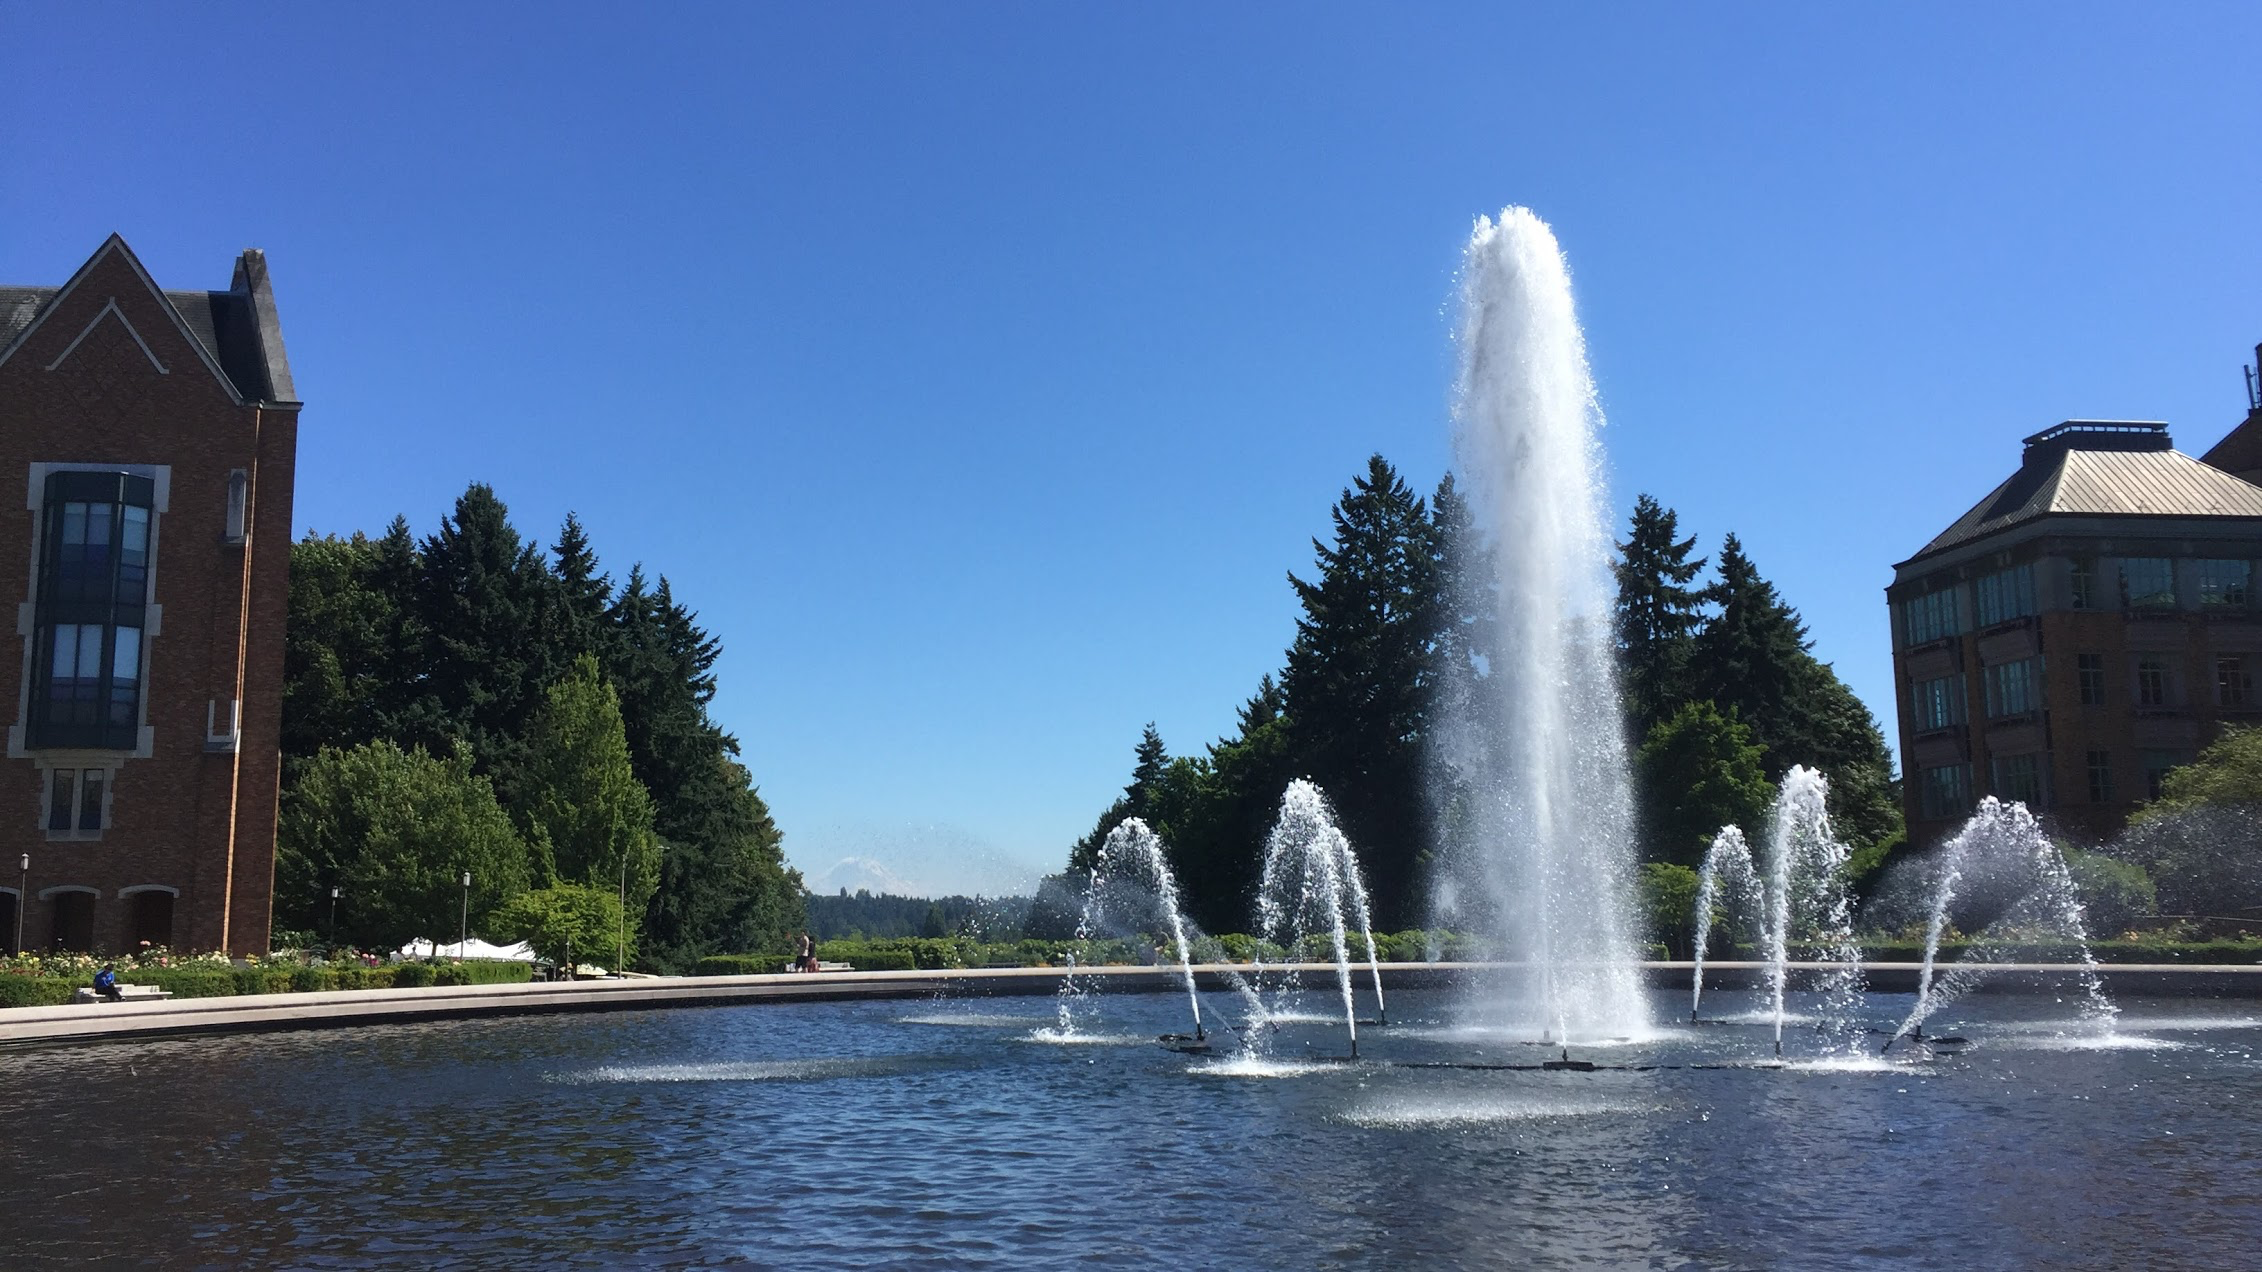
\includegraphics[width=6.0in]{aaafiles/fountain}
%%   \caption{Drumheller Fountain, The University of Washington, Seattle WA.}
%% \end{teaserfigure}

% Processes all of the front-end information and starts the body of the work.
\maketitle

\section{Introduction}


%% \bibliographystyle{ACM-Reference-Format}
%% \bibliography{aaatemplate}
\end{document}
